\subsection{Nanowire with ring segments} \label{subsec:U_wire}

Wide variety of linear and non-linear spin-wave phenomena attracted the interest into the fundamental properties of the spin waves~\cite{Holstein40,Dyson56,Akhiezer68}, whereas their transport abilities are of the great interest for spintronics logical and signal-carrying elements~\cite{Khitun08,Schneider08,Khi10jpd,Vogt12}. Due to the possibility of building compact and low-power logical devices, spin waves are considered as potential data carriers for novel computing devices~\cite{Kruglyak10a,Lenk11,Chumak14,Chumak15,Mahmoud20}. However, in order to exploit spin waves for data processing in real devices, it requires unimpeded spin waves propagation in flat curvilinear structures with complicated geometry. This obliges the use of magnetic waveguides with ring segments of different sizes to preserve save space on chips~\cite{Vogt12,Xing13,Haldar16}, see Fig.~\ref{fig:Circular_segment_1}(a).

\subsubsection{Equilibrium state} \label{subsubsec:U_wire_equilibrium}

Based on Eq.~\ref{eq:Exchange_energy_TNB_2} and general theoretical approach introduced in \ref{sec:model_1D}, let us consider a flat anisotropic ferromagnetic nanowire with a fixed cross-section of area $S$ and localized box-function curvature profile: $\kappa (s) = \kappa_0 \, h(s+s_0) - \kappa_0 \, h(s-s_0)$, see Fig.~\ref{fig:Circular_segment_1}(b) and (c). Here, $h(\xi)$ is the Heaviside step function, $\kappa_0=1/R$ is the curvature of the arc bending with $R$ being the ring segment radius, and $\xi_0 = (\pi-\alpha)R/(2{\ell})$ with $\alpha$ being the expansion angle. To simplify the analytical consideration it is convenient to introduce the angular parameterization of the magnetization in the Frenet-Serret local reference frame, $\vec{m} = \sin\theta \, \cos\phi \, \vec{e}_{\textrm{T}}+\sin\theta \, \sin\phi \, \vec{e}_{\textrm{T}} + \cos\theta \, \vec{e}_{\textrm{B}}$, where the angular variables $\theta $ and $\phi $ depend on spacial and temporal coordinates. In the curvilinear reference frame the total energy \eqref{eq:total_energy} reads 
\begin{equation} \label{eq:Energy-plane}
E = S \, K_\text{eff} \, \int\mathrm{d}\vec{s}\, \left[ \ell^2 \, {\theta'}^2 + \ell^2 \, \sin^2\theta \, \left(\phi'+\kappa\right)^2 - \sin^2\theta\,\cos^2\phi \right],
\end{equation}
where $\ell=\sqrt{\mathcal{A}/K_\text{eff}}$ is the characteristic magnetic length, with $K_\text{eff}=K+\pi M_s^2$ being the constant of the effective easy-tangential anisotropy, that consists of the intrinsic crystalline anisotropy $K$ and the shape-induced magnetostatic contribution~\cite{Gaididei17a}. 

%==================================================================\
\begin{figure*}
	\begin{center}
		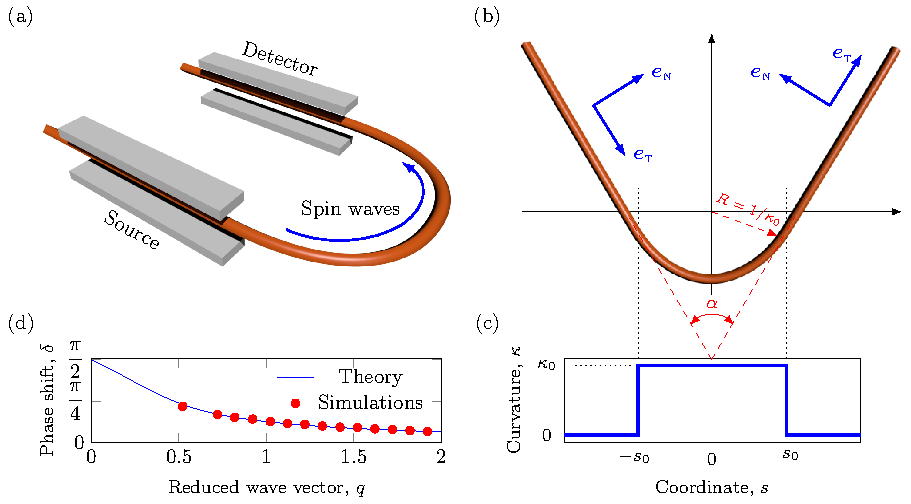
\includegraphics[width=1.0\linewidth]{Circular_segment_1}
	\end{center}
	\caption{
		\textbf{Curved flat ferromagnet wire:} \textbf{(a)}, Schematic of bended ferromagnet wire. The spin wave is generated by an alternating field inside the ``Source'' region and propagates through the bend to  the detector. The phase of the transmitted wave is compared with the phase expected for the straight wire. 
		\textbf{(b)}, Curve with a box-function curvature with $R$ being the bending radius and $\alpha$ being the angle of expansion. 
		\textbf{(c)}, Box-function curvature profile. 
		\textbf{(d)}, Phase shift of the transmitted spin wave according to the \eqref{eq:Levinson} compared with spin-lattice simulations. Adapted with permission from~\cite{Gaididei18a}.}
	\label{fig:Circular_segment_1}
\end{figure*}
%==================================================================/

The equilibrium state of the system corresponds to the minimum of the energy functional \eqref{eq:Energy-plane}: the ground magnetization distribution for the considered wire is also planar and lies in the osculating (TN) plane. Thus, the equilibrium magnetic state has the form 
\begin{subequations} \label{eq:Theta-Phi-statics}
	\begin{equation} \label{eq:gs}
	\Theta = \frac{\pi}{2},\quad \varPhi = \varPhi(s),
	\end{equation}
where the corresponding azimuthal magnetization angle $\varPhi$ is described by the equation of a nonlinear driven pendulum~\cite{Gaididei18a}:
	\begin{equation} \label{eq:LL-statics-phi}
	\ell^2 \, \varPhi '' - \sin\varPhi  \cos\varPhi  = - \ell^2 \, \kappa'.
	\end{equation}
\end{subequations}
In the limiting case of a smoothly curved wire with localized curvature $|\kappa_0| \ll 1/\ell$, the ground state has a form of two hooks in the points of curvature step with exponential tails:
\begin{equation} \label{eq:boxcar-gs-linear}
\varPhi (s) =
\begin{cases}
-\ell \, \kappa_0 \, e^{-s_0/\ell} \, \sinh(s/\ell), & \text{when $|s|\leq s_0$},\\
- \ell \, \kappa_0 \, \text{sgn}(s/\ell) \, e^{-|s/\ell|} \, \sinh(s_0/\ell), &\text{when $|s|> s_0$}.
\end{cases}
\end{equation}

\subsubsection{Magnon eigenmodes and phase shift} \label{subsubsec:U_wire_eigenmodes}

To analyze magnon modes, it is instructive to consider the small deviations of the magnetization vector on the background of the static solution, $\psi=(\theta-\Theta) + i \left(\phi-\varPhi\right)$. This allows to linearize the Landau-Lifshitz equations and rewrite them in the form of a generalized Schr\"odinger equation~\cite{Sheka04,Ivanov05b,Gaididei18a}
\begin{equation} \label{eq:Schroedinger}
-i \,\dot{\psi} = H \, \psi + W \, \psi^\star, \qquad H = -\partial_s^2 +1+V.
\end{equation}
Here the overdot indicates the derivative with respect to the dimensionless time $\tilde{t}=t\omega_0$ with $\omega_0=2\gamma_0K_\text{eff}/M_s$, the star operator means the complex conjugation, and the ``potentials'' have the following form~\cite{Gaididei18a}:
\begin{equation} \label{eq:V-n-W}
\begin{split}
V(s) &= -\frac{1}{2}\left[3\sin^2\varPhi  + \ell^2 \, \left(\varPhi ' + \kappa\right)^2\right],\\
W(s) &= \frac{1}{2}\left[\sin^2\varPhi  - \ell^2 \, \left(\varPhi ' + \kappa\right)^2\right].
\end{split}
\end{equation}
In the case of localized box-function curvature profile, the effective potentials are~\cite{Gaididei18a} 
\begin{equation} \label{eq:V-n-W-as}
V(s) \approx W(s) \approx
\begin{cases}
-\frac{1}{2} \, \ell^2 \, \kappa^2(s), & \text{when $|s|\leq s_0$},\\
0, &\text{when $|s|> s_0$}.
\end{cases}
\end{equation}
Thus, the scattering problem of magnons by the localized bending region becomes equivalent to the scattering problem of a quantum particle inside the potential $V$. Analyzing the generalized Schr\"odinger equation~\eqref{eq:Schroedinger} allows to determine the appearance of local modes (bound states) inside the gap with the frequency~\cite{Gaididei18a} 
\begin{equation} \label{eq:omega-loc}
\omega^{\text{loc}} = \omega_0 \, \left\{1 - \frac{\ell^4}{16} \left[
\int_{-\infty}^{\infty} \kappa^2(s)\mathrm{d}s\right]^2\right\}.
\end{equation}
These local modes are localized on a wire bend and have eigenfrequency below the ferromagnetic resonance $\omega_0$. The interaction of the local modes with spin waves, propagating through the bend, results in a shift of the wave phase according to the quantum scattering theory and the Levinson theorem~\cite{Swan63}. Thus, the total phase shift $\delta_t(0)-\delta_t(\infty)$ is related to the number of bound states (i.e. local modes) $N^{\text{loc}}$ and half--bound states (i.e. half-local modes) $N^{\text{h.loc}}$~\cite{Ma06a}. 
In the 1D case the total phase shift reads~\cite{Dong00b}
\begin{equation} \label{eq:Levinson}
\frac{\delta_t(0)-\delta_t(\infty)}{\pi} = 
\begin{cases}
N_e^{\text{loc}} + \frac12 N_e^{\text{h.loc}} -\frac12, 	& \text{even parity},\\
N_o^{\text{loc}} + \frac12 N_o^{\text{h.loc}}, 			& \text{odd parity}.
\end{cases}
\end{equation}
The resulting scattering phase $\delta_t$ calculated for spin waves propagating through the one-dimensional nanowire with ring segment is plotted in Fig.~\ref{fig:Circular_segment_1}(d).